\documentclass[10pt]{extarticle}
\title{}
\author{}
\date{}
\usepackage[shortlabels]{enumitem}


%paper setup
\usepackage{geometry}
\geometry{letterpaper, portrait, margin=1in}
\usepackage{fancyhdr}
% sans serif font:
\usepackage{cmbright}
%symbols
\usepackage{amsmath}
\usepackage{amssymb}
\usepackage{amsthm}
\usepackage{mathtools}
\usepackage[hidelinks]{hyperref}
\usepackage{gensymb}
\usepackage{multirow,array}
\usepackage{multicol}

\newtheorem*{remark}{Remark}
\usepackage[T1]{fontenc}
\usepackage[utf8]{inputenc}

%chemistry stuff
%\usepackage[version=4]{mhchem}
%\usepackage{chemfig}

%plotting
\usepackage{pgfplots}
\usepackage{tikz}
\tikzset{middleweight/.style={pos = 0.5}}
%\tikzset{weight/.style={pos = 0.5, fill = white}}
%\tikzset{lateweight/.style={pos = 0.75, fill = white}}
%\tikzset{earlyweight/.style={pos = 0.25, fill=white}}

%\usepackage{natbib}

%graphics stuff
\usepackage{graphicx}
\graphicspath{ {./images/} }
\usepackage[style=numeric, backend=biber]{biblatex} % Use the numeric style for Vancouver
\addbibresource{the_bibliography.bib}
%code stuff
%when using minted, make sure to add the -shell-escape flag
%you can use lstlisting if you don't want to use minted
%\usepackage{minted}
%\usemintedstyle{pastie}
%\newminted[javacode]{java}{frame=lines,framesep=2mm,linenos=true,fontsize=\footnotesize,tabsize=3,autogobble,}
%\newminted[cppcode]{cpp}{frame=lines,framesep=2mm,linenos=true,fontsize=\footnotesize,tabsize=3,autogobble,}

%\usepackage{listings}
%\usepackage{color}
%\definecolor{dkgreen}{rgb}{0,0.6,0}
%\definecolor{gray}{rgb}{0.5,0.5,0.5}
%\definecolor{mauve}{rgb}{0.58,0,0.82}
%
%\lstset{frame=tb,
%	language=Java,
%	aboveskip=3mm,
%	belowskip=3mm,
%	showstringspaces=false,
%	columns=flexible,
%	basicstyle={\small\ttfamily},
%	numbers=none,
%	numberstyle=\tiny\color{gray},
%	keywordstyle=\color{blue},
%	commentstyle=\color{dkgreen},
%	stringstyle=\color{mauve},
%	breaklines=true,
%	breakatwhitespace=true,
%	tabsize=3
%}
% text + color boxes
\renewcommand{\mathbf}[1]{\mathbold{#1}}
\usepackage[most]{tcolorbox}
\tcbuselibrary{breakable}
\tcbuselibrary{skins}
\newtcolorbox{problem}[1]{colback=white,enhanced,title={\small #1},
          attach boxed title to top center=
{yshift=-\tcboxedtitleheight/2},
boxed title style={size=small,colback=black!60!white}, sharp corners, breakable}
%including PDFs
%\usepackage{pdfpages}
\setlength{\parindent}{0pt}
\usepackage{cancel}
\pagestyle{fancy}
\fancyhf{}
\rhead{Avinash Iyer}
\lhead{Math 212: Homework 7}
\newcommand{\card}{\text{card}}
\newcommand{\ran}{\text{ran}}
\newcommand{\N}{\mathbb{N}}
\newcommand{\Q}{\mathbb{Q}}
\newcommand{\Z}{\mathbb{Z}}
\newcommand{\R}{\mathbb{R}}
\begin{document}
  \begin{problem}{16.2}
    \begin{description}[font=\normalfont]
      \item[2:] \hfill
        \begin{center}
          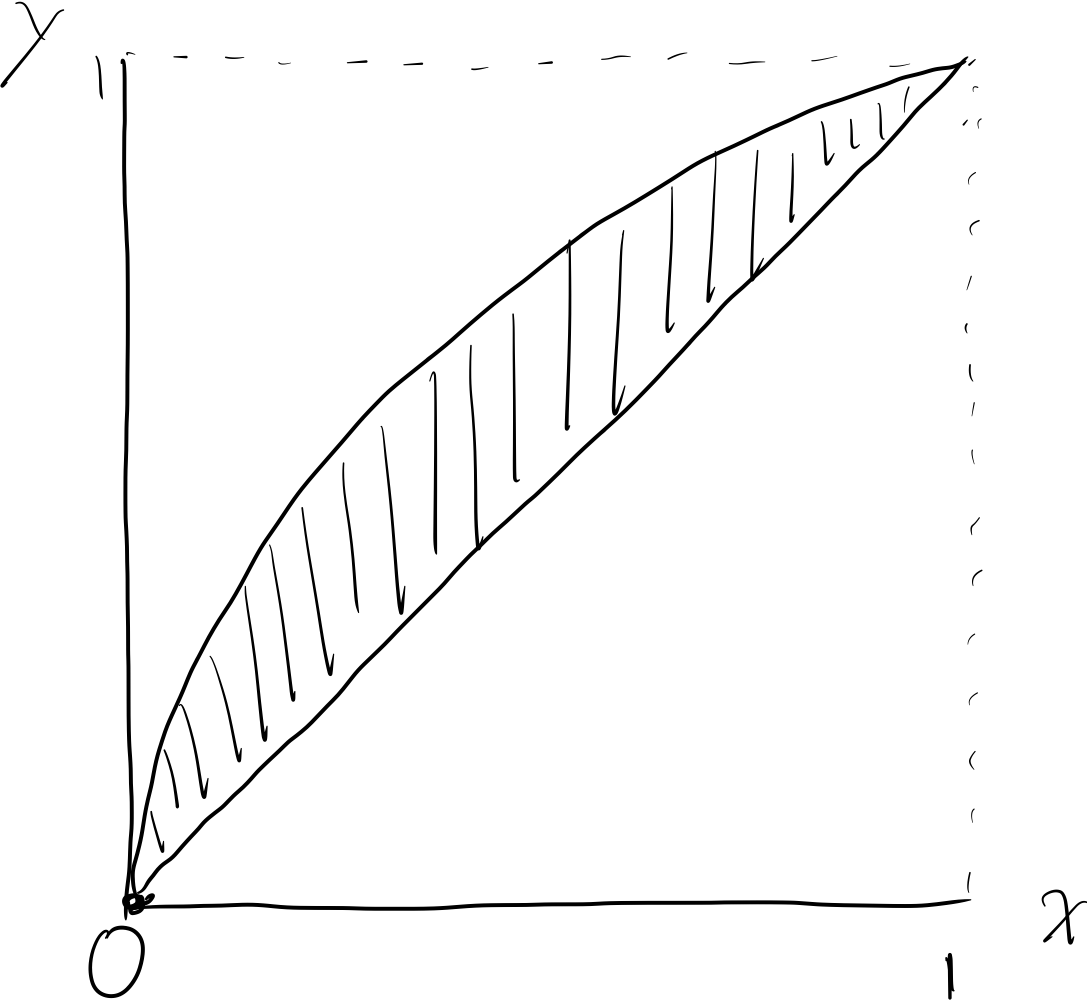
\includegraphics[height=0.5\textwidth]{images/16_2_2.png}
        \end{center}
      \item[4:]\hfill
        \begin{center}
          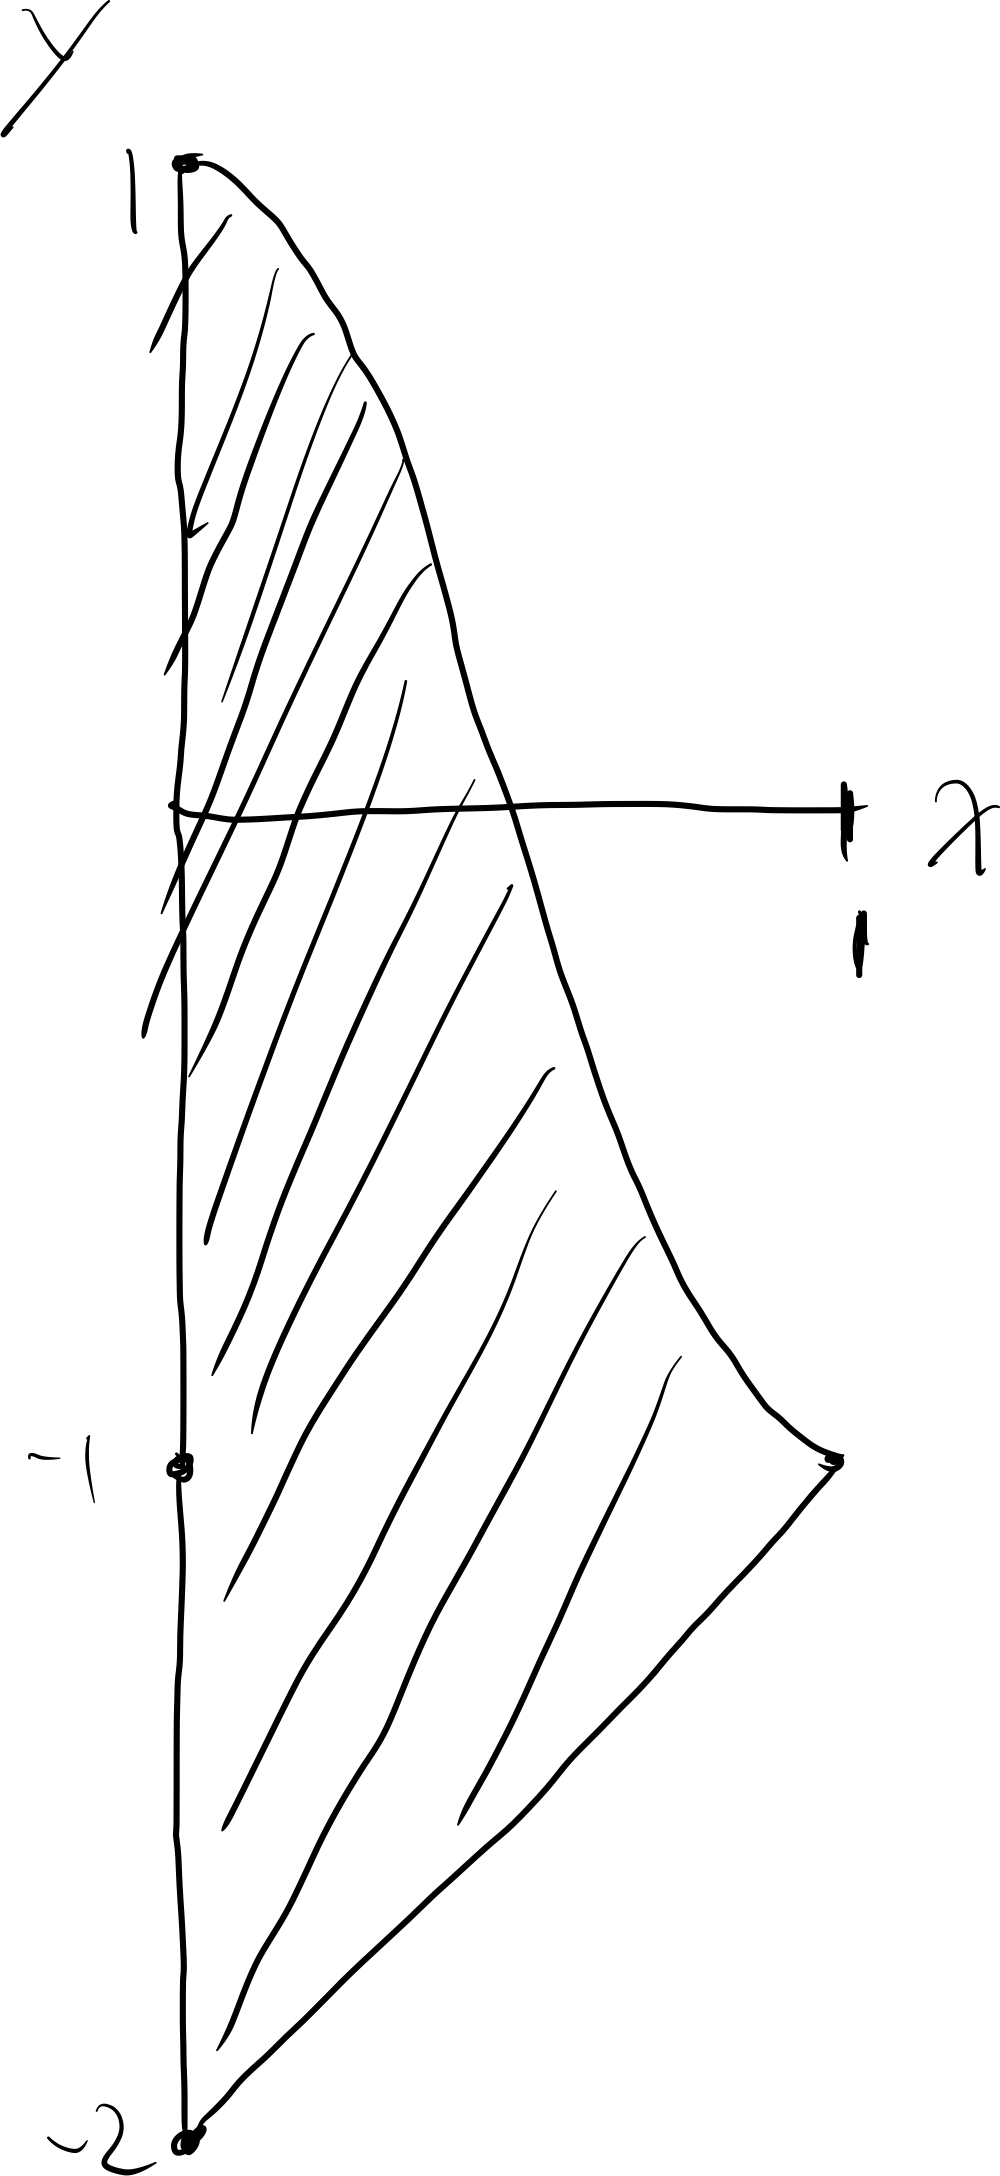
\includegraphics[height=0.5\textwidth]{images/16_2_4.png}
        \end{center}
      \item[6:]
        \begin{align*}
          \int_{0}^{2}\int_{0}^{3}(x^2 + y^2)~dy~dx &= \int_{0}^{2}\left(x^2y + \frac{y^3}{3}\biggr\vert_{y=0}^{y=3}\right)~dx\\
                                                    &= \int_{0}^{2}\left(3x^2 + 9\right)~dx\\
                                                    &= x^3 + 9x\biggr\vert_{0}^{2}\\
                                                    &= 26
        \end{align*}
      \item[12:]
        \begin{align*}
          \int_{0}^{\pi/2}\int_{0}^{\sin x}x~dy~dx &= \int_{0}^{\pi/2}\left(xy\biggr\vert_{y=0}^{y=\sin x}\right)~dx\\
                                                   &= \int_{0}^{\pi/2}x\sin x~dx\\
                                                   &= \sin x - x\cos x\biggr\vert_{0}^{\pi/2}\\
                                                   &= 1
        \end{align*}
      \item[14:]\hfill
        \begin{center}
          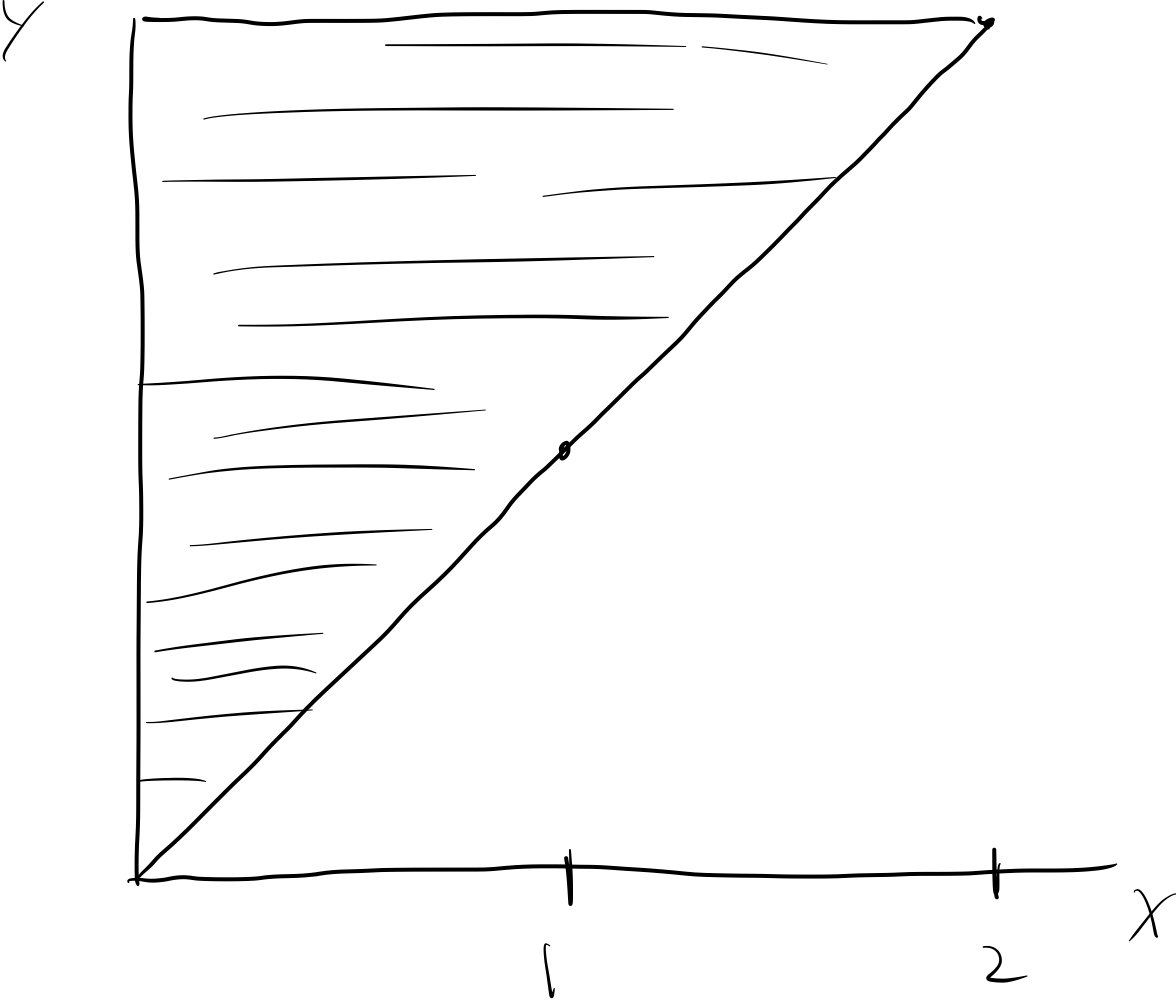
\includegraphics[height=0.5\textwidth]{images/16_2_14.png}
        \end{center}
        \begin{align*}
          \int_{0}^{2}\int_{0}^{x}e^{x^2}~dy~dx &= \int_{0}^{2}\left(ye^{x^2}\biggr\vert_{y=0}^{y=x}\right)~dx\\
                                                &= \int_{0}^{2}xe^{x^2}~dx\\
                                                &= \frac{1}{2}\int_{0}^{4}e^{u}~du \tag*{$u = x^2,~du = 2x~dx$}\\
                                                &= \frac{1}{2}\left(e^4 - 1\right)
        \end{align*}
      \item[20:]
        \begin{center}
          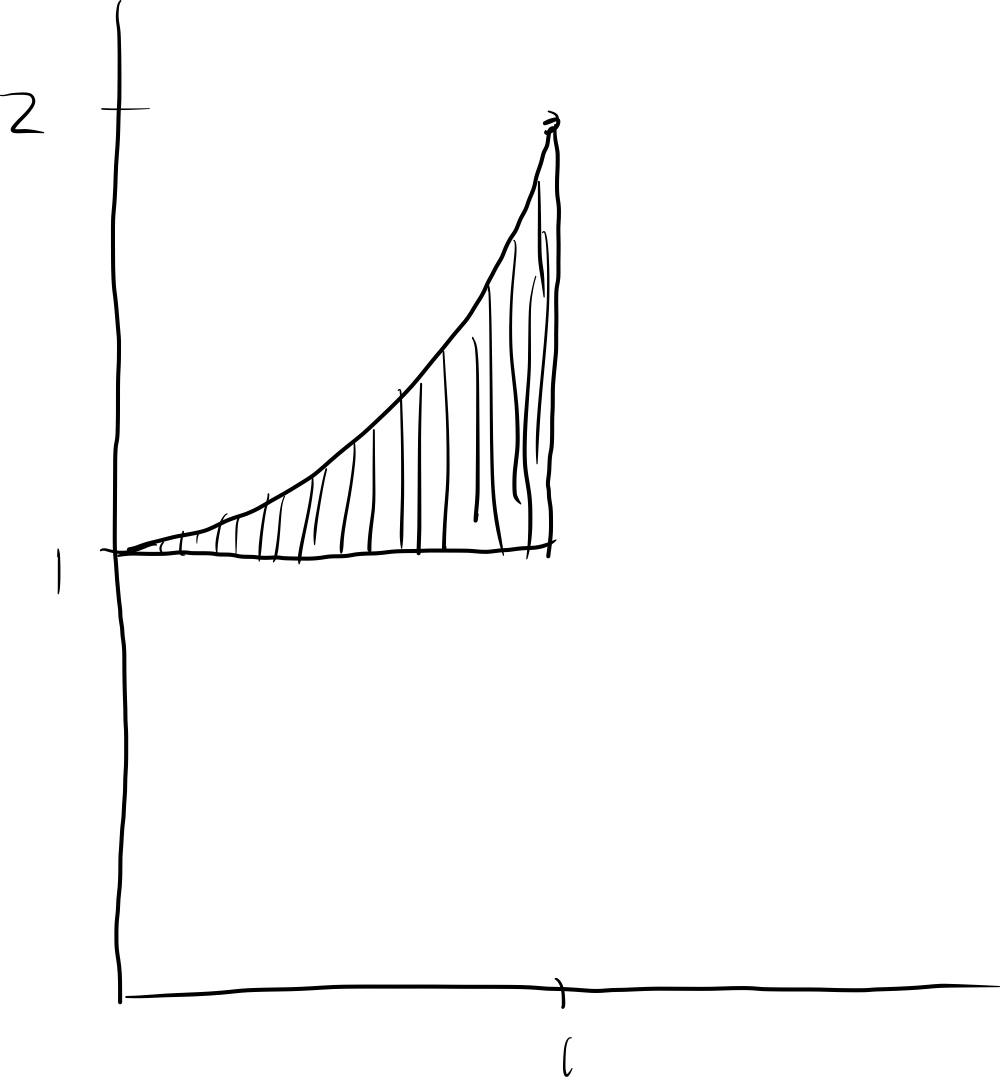
\includegraphics[height=0.5\textwidth]{images/16_2_20.png}
        \end{center}
        \begin{align*}
          \int_{0}^{1}\int_{1}^{1 + x^2}\frac{x}{\sqrt{y}}~dy~dx &= \int_{0}^{1}\left(2x\sqrt{y}\biggr\vert_{1}^{1 + x^2}\right)~dx\\
                                                                 &= \int_{0}^{1}2x\sqrt{1 + x^2}~dx - \int_{0}^{1}2x~dx\\
                                                                 &= -\frac{1}{2} + \int_{1}^{2}\sqrt{u}~du\tag*{$u = 1 + x^2,~du = 2x~dx$}\\
                                                                 &= -\frac{1}{2} + \frac{2}{3}\left(u^{3/2}\biggr\vert_{1}^{2}\right)\\
                                                                 &= -\frac{1}{2} + \frac{2}{3}\left(2\sqrt{2} - 1 \right)\\
                                                                 &= \frac{1}{3}\left(-5 + 4\sqrt{2}\right)
        \end{align*}
      \item[24:]
        \begin{align*}
          \int_{0}^{6}\int_{y/2}^{y/3+5}f(x,y)~dx~dy
        \end{align*}
      \item[26:]
        \begin{align*}
          \int_{1}^{4}\int_{x/3-1/3}^{2}f(x,y)~dy~dx
        \end{align*}
      \item[44:]
        \begin{align*}
          \int_{0}^{1}\int_{y}^{1}\sin(x^2)~dx~dy &= \int_{0}^{1}\int_{0}^{x}\sin(x^2)~dy~dx\\
                                                  &= \int_{0}^{1}x\sin(x^2)~dx\\
                                                  &= \frac{1}{2}\sin(1)
        \end{align*}
      \item[46:]
        \begin{align*}
          \int_{0}^{3}\int_{y^2}^{9}y\sin(x^2)~dx~dy &= \int_{0}^{9}\int_{0}^{\sqrt{x}}y\sin(x^2)~dy~dx\\
                                                     &= \frac{1}{2}\int_{0}^{9}x\sin(x^2)~dx\\
                                                     &= \frac{1}{4}\sin(81)
        \end{align*}
    \end{description}
  \end{problem}
  \begin{problem}{16.3}
    \begin{description}[font=\normalfont]
      \item[2:]
        \begin{align*}
          \int_{0}^{1}\int_{0}^{1}\int_{0}^{2} ax+by+cz~dz~dy~dz &= \int_{0}^{1}\int_{0}^{1} 2ax+2by+2c~dy~dx\\
                                                                 &= \int_{0}^{1}2ax + b + 2c~dx\\
                                                                 &= a + b + 2c
        \end{align*}
      \item[4:]
        \begin{align*}
          \int_{0}^{a}\int_{0}^{b}\int_{0}^{c}e^{-x-y-z}~dz~dy~dz &= \int_{0}^{a}\int_{0}^{b}e^{-x-y-z}\left(e^{-c}-1\right)~dy~dz\\
                                                                  &= \int_{0}^{a}e^{-x-y-z}\left(e^{-b}-1\right)\left(e^{-c}-1\right)~dx\\
                                                                  &= \left(e^{-a}-1\right)\left(e^{-b} - 1\right) \left(e^{-c} - 1\right)
        \end{align*}
      \item[6:]
      \item[16:] Positive.
      \item[18:] Zero.
      \item[24:] Zero.
      \item[26:] Positive.
    \end{description}
  \end{problem}
  \begin{problem}{16.4}
    \begin{description}[font=\normalfont]
      \item[2:]
        \begin{align*}
          \int_{0}^{\sqrt{2}}\int_{0}^{2\pi}f(r,\theta)r~d\theta~dr
        \end{align*}
      \item[4:]
        \begin{align*}
          \int_{1}^{2}\int_{\pi/2}^{3\pi/2}f(r,\theta)r~d\theta~dr
        \end{align*}
      \item[10:]\hfill
        \begin{center}
          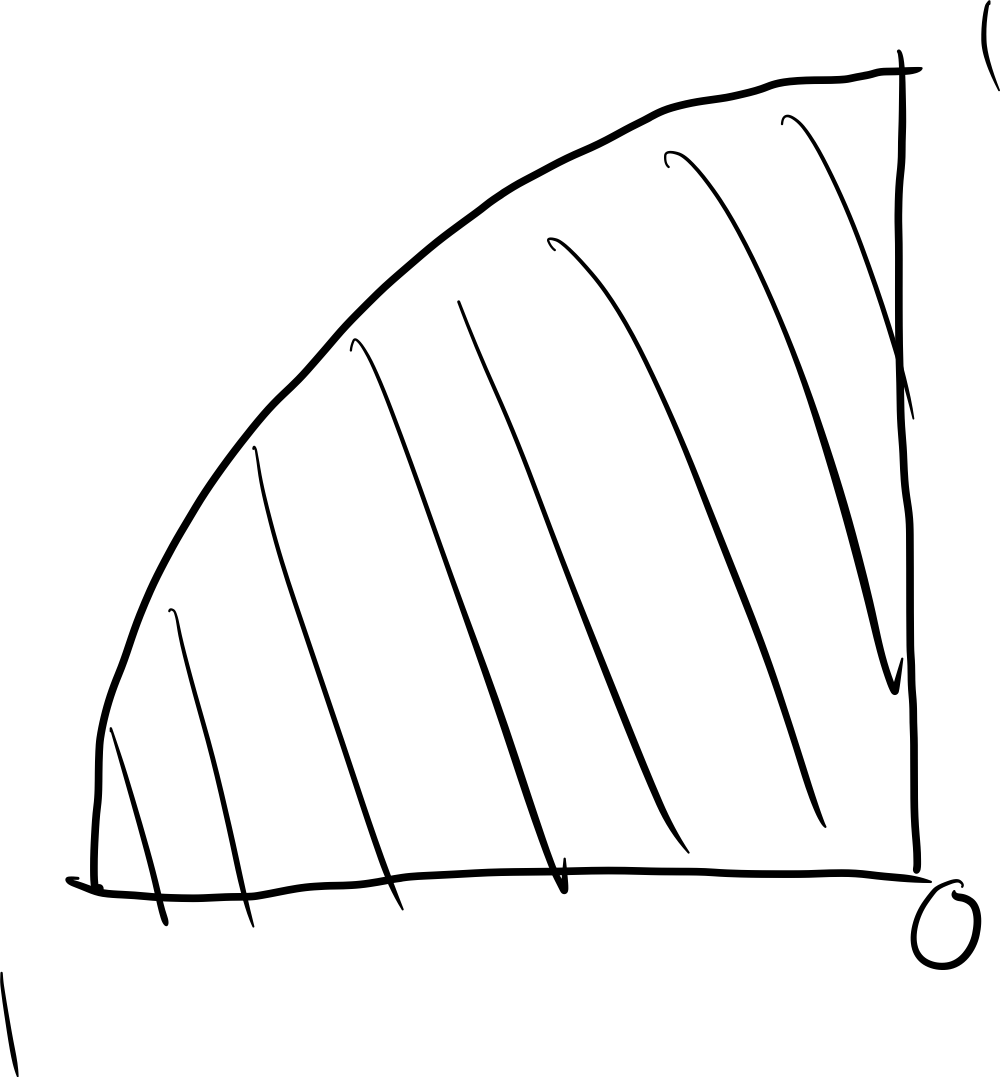
\includegraphics[height=0.5\textwidth]{images/16_4_10.png}
        \end{center}
      \item[12:]\hfill
        \begin{center}
          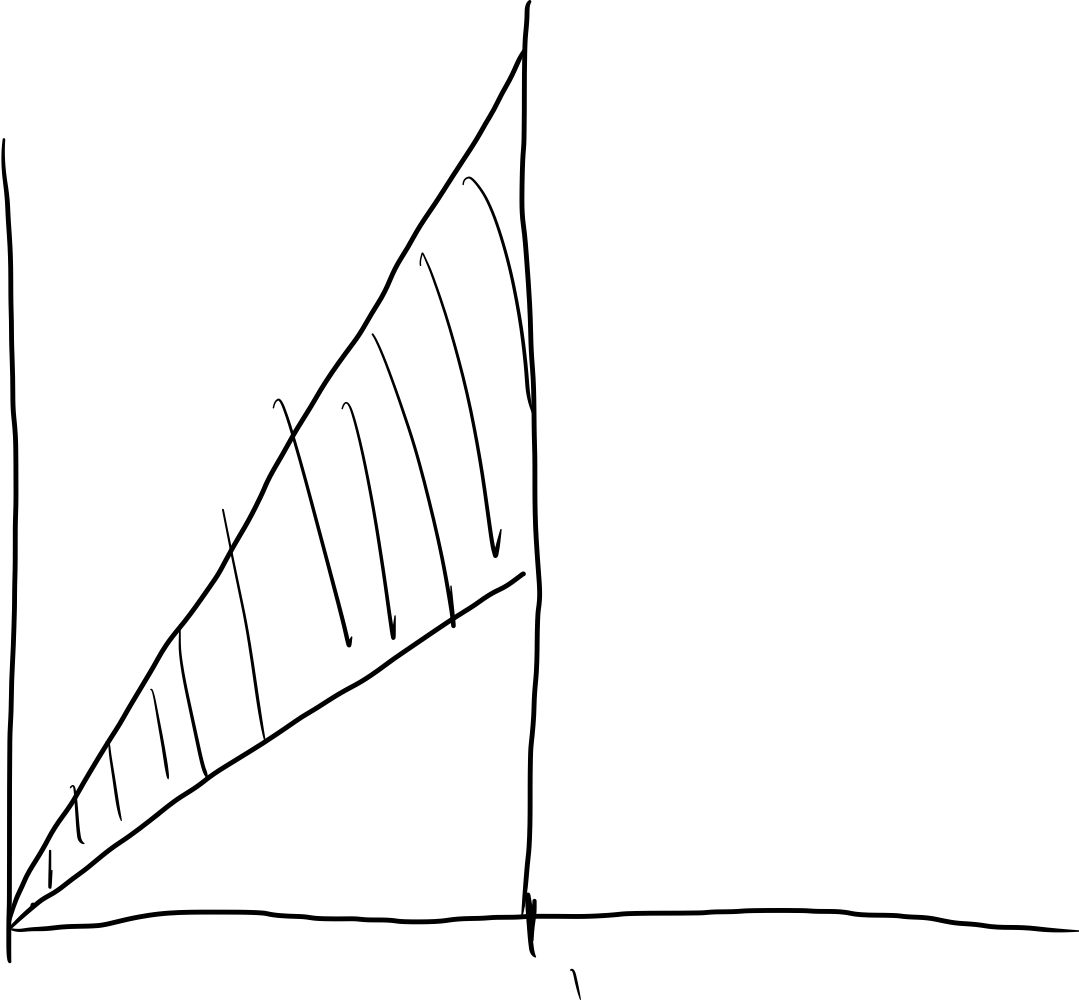
\includegraphics[height=0.5\textwidth]{images/16_4_12.png}
        \end{center}
      \item[16:]
        \begin{align*}
          \int_{R}\sqrt{x^2 + y^2}~dx~dy &= \int_{0}^{\pi/2}\int_{2}^{3}r^2~dr~d\theta\\
                                         &= \frac{1}{3}\int_{0}^{\pi/2}19~d\theta\\
                                         &= \frac{19\pi}{6}
        \end{align*}
      \item[20:] I don't know how to do this problem.
      \item[32:]
        \begin{align*}
          \int_{0}^{2\pi}d\theta\int_{0}^{\sqrt{8}}rdr\int_{0}^{8-r^2}dz &= 2\pi\int_{0}^{\sqrt{8}}r\sqrt{8-r^2}dr\\
                                                                         &= \frac{32\sqrt{2}}{3}\pi
        \end{align*}
    \end{description}
  \end{problem}
  \begin{problem}{16.5}
    \begin{description}[font=\normalfont]
      \item[2:]
        \begin{align*}
          A &= \{r,\theta,z\mid r\in(-\infty,\infty),~\theta=\pi/4,~z\in(-\infty,\infty)\}
        \end{align*}
      \item[4:]
        \begin{align*}
          z &= r\\
          r&\in(0,\infty)\\
          \theta&\in[0,2\pi)
        \end{align*}
      \item[6:] 
        \begin{align*}
          z &= 10
        \end{align*}
      \item[8:]
        \begin{enumerate}[(a)]
          \item Cone and Sphere respectively.
          \item $z = r$ and $z^2 + r^2 = 1$
          \item An ice cream cone.
          \item $2r^2 = 1$
          \item $2(x^2 + y^2) = 1$
        \end{enumerate}
      \item[10:]
        \begin{align*}
          \int_{W}f(x,y,z) &= \int_{-3}^{1}\int_{0}^{2\pi}\int_{0}^{1}\sin(r)~dr~d\theta~dz\\
                           &= 8\pi(1-\cos 1)
        \end{align*}
    \end{description}
  \end{problem}
\end{document}
